\chapter{Multimodal Fuzzy Fusion Framework for Semantic Video Indexing Improvement}
\label{c1}

		%The availability of large-scale video annotated datasets constitutes a crucial requirement 
		%for promoting knowledge discovery. Many annotation tools were provided \citep{Dasiopoulou2011}
		%(such as \emph{VIA}, \emph{VideoAnnEx}, \emph{Ontolog}, \emph{Advene}, \emph{Elan}, \emph{Anvil},
		% \dots). These tools investigate spatial-temporal information in a video content. However,
		%no standardized large-scale annotated video dataset was officially proposed. Particularly, 
		%\textsc{TrecVid} \cite{Over2013} proposed a standardized annotated video dataset used for
		%measuring video retrieval and indexing performances. 

	

	In this chapter, we detail and discuss the first contribution $C_{1}$. In fact, we propose a general 
	multimodal fuzzy approach to enhance video semantic indexing accuracy. The latter approach was developed 
	incrementally through some consecutive research works. For that, and in the section \ref{c1_1}, 
	we first introduce our preliminary reflections for a knowledge based framework to index video content 
	efficiently. Then, in section \ref{c1_2}, and based on what was obtained through an experimental study, 
	we present a framework improvement, in particular, handling fuzzy knowledge and corresponding reasoning 
	ability. Finally, in section \ref{c1_3}, we present our proposed video annotation tool in order to generate 
	valuable data source about video content. First of all, section \ref{c1_0} displays first \revAnglais{afterthought}
	for a knowledge based video indexing framework.

	\section{Context and Motivation}
	\label{c1_0}

	Multi-modal fusion has gained much attention by the multimedia community \citep{Atrey2010}. 
	In fact, a video indexing task involves processing of multi-modal data in order to obtain valuable 
	insights about the content. Such a task could use sensory data (such as audio and visual analysis) 
	as well as \revAnglais{non-sensory} data (such as meta-data). Thus, the fusion of multiple modalities can provide 
	complementary information and increase, then, the accuracy of the indexing process.
	
	In \citep{Lucien1999}, the data fusion is defined as follows:
		\begin{definition}
			''a formal framework in
 		which are expressed means and tools for the alliance of
 		data originating from different sources. It aims at obtaining
 		information of greater quality''.
	\end{definition}

	A discussed in \citep{Waltz1990,Esteban2005,Blasch2006,Guerrero2009}, a fusion process 
	consists of five levels: The \emph{level 0} (named  \emph{pre-processing}) and \emph{level 1}
	(named \emph{object refinement}) cover respectively signal processing and data alignment. 
	The \emph{level 2} (named \emph{situation refinement}) attempts to \revAnglais{construct} a complete picture 
	from incomplete information provided by the lower levels (\emph{level 0} and \emph{level 1}).
	The \emph{level 3} (named \emph{threat refinement}) interprets the results from \emph{level 2} 
	in terms of the possible opportunities for operation. A \emph{process refinement},
	referred to \emph{level 4}, loops around these earlier levels to monitor performance 
 	and optimize the fusion process. Earlier data fusion applications were initially used for
	military reasons. But currently, data fusion model is extended for several other 
	areas \citep{LigginsII2008}.

	By drawing inspiration from this fusion model, we propose a fusion framework to fuse 
	multi-modal video content extracted semantics (concepts). Thus, we adopt the
	\textsc{Jdl/Dfs} data fusion model \citep{Waltz1990}.

	After an experimental study carried out within \textsc{TrecVid2010} evaluation campaign,
	we concluded that the multi-modal fusion process is important, but a big challenge occurred on 
	how to efficiently manage and explore fuzzy knowledge for better semantic indexing enhancement. 
	From this observation, we decided to tackle in depth the knowledge management raised issue. 
	Thus, we proposed a preliminary fuzzy ontology based framework to explore knowledge reasoning 
	capabilities in video indexing. A light ontology structure was proposed, as well as \revAnglais{an} abduction 
	engine to extract fuzzy knowledge from valuable data sources, and a deduction engine able to 
	leverage from the extracted knowledge in order to generate newer knowledge filling out a semantic
	interpretation about a video content.

	Yet again, the experimental study showed that the use of contextual ontologies has improved 
	the indexing process performances, however good, a simple set of manually defined contexts 
	were used. Aiming to go further in the use of contextual information, we proposed afterwards 
	a fuzzy video collaborative annotation tool that helps to detect potential semantic concept 
	inter-relationships. The latter are important to define semantic contexts.
		
	In the following section, we display in details main works that have been conducted 
	in order to \revAnglais{realize} our first contribution $C_{1}$.
	
	\section{A Multimodal Fuzzy Fusion Framework}
	\label{c1_1}

	
	In this section, we will introduce our fusion system and
	describe the multi-modal fuzzy fusion process.

	The proposed fusion architecture, based on the JDL/DFS model, is shown in figure \ref{fig:contrib1::fig1}. 
	After extracting unimodal semantic interpretation (level 0), the level 1 
	is called to search and eliminate conflicting situations. Then, level 2 
	is applied on level 1 results aiming at finding further concepts based 
	on abduction and deduction engines. These engines analyses relationships
	between concepts. The level 4 is used to control the whole fusion process. 
	Below is the description of the different integrated levels and the proposed fusion architecture.
	
	\begin{figure}[ht!]	
		\centering
		\includegraphics[width=\textwidth]{graphics/contrib1::fig1}
		\caption{Overview of the proposed Multimodal Fuzzy Fusion System}
		\label{fig:contrib1::fig1}
	\end{figure}

	\subsection{Object refinement (level 1)}
		The \emph{level 1} deals with mixed unimodal semantic interpretations. The latters are structured through 
		this data \revAnglais{format:} every concept has a list of indexed video content sorted by their descending 
		pertinent ranks. These ranks are fuzzified then analyzed.
		
		\begin{description}
			\item[Concept ranks fuzzification]
			The purpose of this step is to calculate the fuzzy membership
			degree of a concept to a video content. 
			This is given by a normalization function (see equation \ref{equation1}).

			Let $r$ be the rank of a concept for a video content, and $R$ is the highest 
			rank of the same concept for all video contents. We seek for a transformed rank called $r_{N}$ as follows:
			\begin{equation}
				\label{equation1}
				r_{N} = \left( \frac{(\epsilon -1)}{(R-1)} * (R-r) \right) +1 
			\end{equation}
			Where $\epsilon$ is a \revAnglais{positive} integer.

			\item[Conflicting situations handling]
		Sometimes, certain conflicting situations can be found in aggregated semantic interpretations.
		Since we are using fuzzy logic, two contradictory semantic interpretations can coexist for the 
		same video content. This situation is  permitted until the equation \ref{equation2} is verified.
		
		Let $c_{1}$ and $c_{2}$ be two contradictory concepts. And Let $\mu(c_{1})$ and $\mu(c_{2})$
		be respectively the relevance degree of the first and the second concepts. 

		\begin{equation}
			\label{equation2}
				\Big((1 - \mu(c_{1})) - \epsilon \Big)   \leq   \mu(c_{2})   \leq    
				\Big( (1 - \mu(c_{1})) + \epsilon \Big) 
		\end{equation}
		Where $\epsilon$ is a \revAnglais{positive} integer.
		
		If the equation is not verified, the concept, extracted from the less 
		confident modality, is deleted. This trust degree is established for each modality by the fusion 
		control process (\emph{level 4}).

		\end{description}

		In other situations, we find that the concept relevance analysis in a video content varies from one 
		modality to another. This conflict over the relevance degree for the same concept is solved using the equation 
		\ref {equation3}. (Same equation used in \citep{Vrochidis2010}).

		Let $c$ a concept. And let $\mu_{1}(c)$ and $\mu_{2}(c)$  the relevance degrees computed repectively from the 
		first and the second modalities.

		\begin{equation}
			\label{equation3}
			\mu(c) = \alpha \mu_{1}(c)  + \beta \mu_{2}(c)
		\end{equation}
		Where $\alpha$ and $\beta$ are trust degrees respectively for the first and second modalities fixed by 
		the fusion process control (\emph{level 4}), and $\alpha + \beta = 1$.

		We can recognize that level 1 has a great importance since it eliminates any irrelevant information. 
		However, several actual indexing systems do not account well for this component (as in \citep{Vrochidis2010},
		\citep{Snoek2006} and \citep{Ayache2007}).

		The set of fuzzyfied and filtered concepts are finally passed to \emph{level 2}.

	\subsection{Situation refinement (\emph{level 2})}
		The purpose of this level is to look for new concepts by \revAnglais{analyzing} available interpretations.
		To do this, we propose the use of two different intelligent techniques:

		\subsubsection{Deduction engine}
		Using a Mamdani fuzzy system \citep{Mamdani1975},
		 a deduction engine infers new concepts using fuzzy rules extracted from the LSCOM ontology \citep{Kennedy2006}. 
		This ontology is based on generalization relationships. Figure \ref{lscom} illustrates how we extract automatically
		fuzzy rules from the LSCOM ontology.

		Since the concept relevance degrees are already fuzzifyed, we don't need to use the fuzzification 
		(first component of the Mamdani fuzzy system).
		The defuzzification component is also not used.
		
		Our deduction engine is similar to the network of operators described in \citep{Ayache2007}. 
		The main difference between the two systems is that our system extracts the rules automatically 
		from the analysis of an ontology, but the network of operators is set manually. 
		The second difference is that our system deals with fuzzy interpretations.

		Figure \ref{deduction} shows an overview of the deduction engine using extracted fuzzy rules.
		\begin{figure}[h]
			\centering
			\includegraphics[scale=0.45]{graphics/contrib1::lscom_example}
			\caption{Extracting Fuzzy Rules from LSCOM Ontology}
			\label{lscom}
		\end{figure}

		\begin{figure}[h]
			\centering
			\includegraphics[scale=0.45]{graphics/contrib1::deduction}
			\caption{Deduction engine for situation refinement}
			\label{deduction}
		\end{figure}
		
		\subsubsection{Abduction engine}
		The abduction engine is based on a learning system that allows analysis of a  learning video database 
		in order to find possible relationships between concepts as input and expected concepts as output.
		These relationships are then considered  as fuzzy rules used for the deduction of new concepts based 
		on extracted ones from a test video database. Figure \ref{abduction} illustrates an overview of the abduction 
		engine.

		This engine uses the $\beta{}eta$ fuzzy systems (\emph{BFS}) based on a multi-agent genetic algorithm \citep{Kallel2006}.
		Thus, we use the equation \ref{genetic} for minimizing objective function $obj\_fun$ and then, 
		optimizing the learning process.
		
		Let $C$ be a set of $n$ concepts: $C = \{c_{1}, c_{2}, \dots, c_{n}\}$.
		And let $\mu'(c_{i})$ and $\mu''(c_{i})$ be two relevant degrees of the concept $c_{i}$ to a video content 
		respectively for generated concepts as output and the expected ones.
		We compute the objective function $obj\_fun$ by this equation:

		\begin{equation}
			\label{genetic}
			obj\_fun = \frac{\sum_{i=1}^{n} \Big(\mu''(c_{i}) - \mu'(c_{i})\Big)}{\sum_{i=1}^{n}(\mu''(c_{i}))^2}
		\end{equation}
		
		
		A similar abduction engine is described in \citep{Snoek2006} using \revAnglais{a} supervised \emph{SVM} classifier. 
		This latter consists in \revAnglais{analyzing} a set of concepts to discover potential relationships.

		We note that the output of \emph{level 2} is the fusion of two outputs from the deduction and abduction engines. 
		Eventual conflicting situation are treated in the same way as used in the \emph{level 1}. The degree of trust 
		for each reasoning engine is fixed by the fusion control process (\emph{level 4}).
		\begin{figure}[h]
			\centering
			\includegraphics[scale=0.45]{graphics/contrib1::abduction}
			\caption{Abduction engine for situation refinement}
			\label{abduction}
		\end{figure}
		
	\subsection{Fusion Process Control (\emph{level 4})}
		This level aims at controlling the fusion process by manipulating trust  degree of each modality 
		(text, sound and images) and for each reasoning  engine (abduction and deduction). These trust degrees 
		are determined according to a supervised learning.

	We can conclude that the proposed multimodal fuzzy fusion is \revAnglais{characterized} \revAnglais{by} its ability to deliver 
	a rich and coherent semantic interpretation. This is mainly due to:
	\begin{itemize}	
		\item the use of fuzzy logic and fuzzy reasoning,
		\item a  maximum compatibility with the \emph{JDL/DFS} data fusion model,
		\item operating a maximum information  extracted from a video content (multimodality).
	\end{itemize}
	
	However, the quality of this fusion system is still dependent on the quality of initial semantic interpretations delivered by 
	unimodal analyzers.

	
	\subsection{Experimental Study}
		In order to illustrate the semantic enhancement of concept detection introduced 
		by our proposed fuzzy \revAnglais{fusion and} ontology-based framework, we have conducted two preliminary experiments 
		within two 
		multimedia evaluation campaigns. Hence, we expose the experimental setup and the 
		obtained results of our framework within \textsc{Trec} Video Retrieval Evaluation 2010 (\textsc{TrecVid 2010}) 
		\citep{Over2010} at the \textit{Semantic Indexing} task.
		

		\subsubsection{Datasets Description}
		We used datasets provided 
		in \textsc{TrecVid 2010} benchmark. The \textsc{TrecVid 2010} \textit{Semantic Indexing} task provides 
		two datasets proposed by the National Institute of Standards and Technology (\textsc{Nist}): 
		a test and a development dataset. 
		The development dataset (\emph{IACC.1.tv10.training}) contains $3200$ Internet Archive videos 
		($50GB$, $200 h$), while the test dataset (\emph{IACC.1.A}) contains approximately $8000$ Internet 
		Archive videos ($50GB$, $200 h$). The development dataset is annotated by $130$ semantic concepts.


		\subsubsection{Evaluation metrics}
		In order to be able to compare different indexing approaches, various system 
		effectiveness metrics have been used. These metrics are commonly based on precision
		(which is defined as the number of relevant answers as a part of the total number
		of retrieved ones), and recall (which is defined as the number of relevant answers
		as part of total relevant ones in the collection). In our experiments, we consider the following
		evaluation measures:  the \emph{Inferred Average Precision} (\textit{infAP}), the \emph{precision}
		(\textit{P}) and the recall (\textit{R}) as a
		performance metric for the \textsc{TrecVid 2010} \textit{Semantic Indexing} task.

		\subsubsection{Experiments with \textsc{TrecVid 2010} dataset}
		As an earlier experiment, we participated in \textsc{TrecVid 2010} 
		with two runs \textbf{\textit{$Regim_{4}$}} and  \textbf{\textit{$Regim_{5}$}} \citep{Elleuch2010}. 
		The first run integrates only a visual semantic concept detector using key-points detection 
		and visual features extraction tools \citep{Elleuch2010b}. And the second run aims at enhancing indexing 
		effectiveness of the first one through a rule based deduction reasoning engine.  
		Then, only the deduction process is used in the  \textbf{\textit{$Regim_{5}$}} run. 
		The abduction engine is ignored since a set of rules 
		\footnote{http://www-nlpir.nist.gov/projects/tv2010/tv10.semantic.indexing.relations2.txt} 
		were defined manually from the LSCOM ontology \citep{Kennedy2006}. 
		This rule list is based on two potential relationships between two concepts: 
		\emph{implies} (111 rules) and \emph{excludes} (5 rules). 
		For instance, the rule \textit{``Sky \textbf{implies} Outdoor''} depicts that if the concept 
		\textit{Sky} exists in a shot, then the concept \textit{Outdoor} exists too. 
		Similarly, the rule \textit{``Single\_Person \textbf{excludes} Crowd''} depicts that if the concept 
		\textit{Single\_Person} is detected in a shot, then the concept \textit{Crowd} doesn't exist.
		In our case, we \revAnglais{considered} only \textit{\textbf{implies}} relationships based rules.

		The results of both $regim_{4}$ and $regim_{5}$ are shown in figures \ref{res1tervcid2010} and
		\ref{trecvid20102}.
		The $regim_{5}$ run presents a concept detection enhancement over a classical visual concept 
		detector for concepts 6,  15 and 126 (respectively the concepts: \textit{Animal}, \textit{Boat\_Ship} and  
		\textit{Vehicle}). Further, the \textit{$regim_{5}$} run achieved an enhancement of $4.8\%$ for the mean inferred average
		precision (\textit{\textbf{infAP}}=$0.089$) among the \textit{$regim_{4}$} run (\textit{\textbf{infAP}}=$0.085$).
		Thus, having regard to a weak set of rules used in the deduction engine, 
		a knowledge based concept detection enhancement looks promising. Additionally, not all the concept set (130) 
		\revAnglais{were} considered in the rule list. 
		We would like also to point out that the \textsc{TrecVid 2010} evaluation process
		gave concept detection performances for only 30 concepts (among 130). 
		Thus, handling more concepts in the rule list should lead to a better semantic enhancement.

		\begin{figure*}[ht!]	
			\centering
			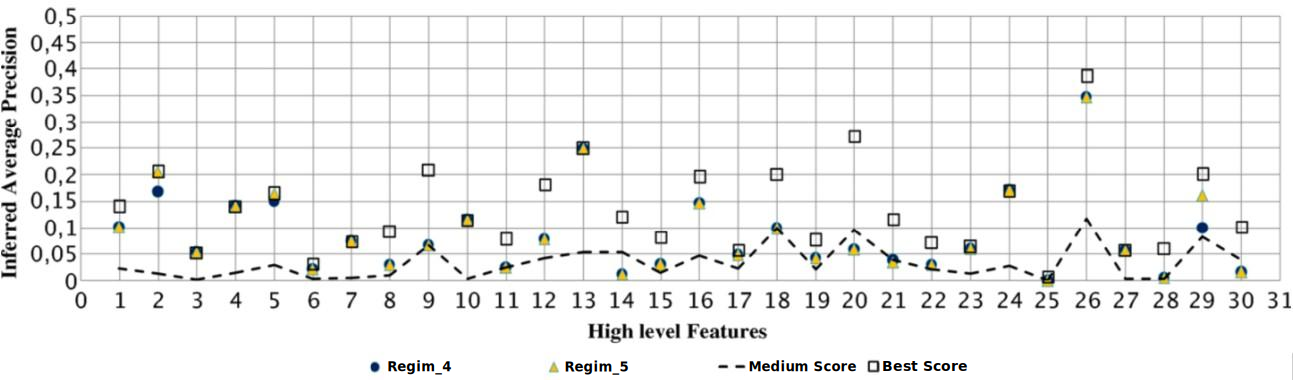
\includegraphics[width=\textwidth]{graphics/trecvid3}
			\caption{\textsc{TrecVid 2010}: $regim_{4}$ and $regim_{5}$ runs evaluations}
			\label{res1tervcid2010}
		\end{figure*}

		\begin{figure}[ht]
			\centering
			\includegraphics[scale=0.4]{figures/trecvid2010_2}
			\caption{\textsc{TrecVid 2010}: $regim_{5}$ ranking in  \textsc{TrecVid 2010} Semantic Indexing Task (SIN)}
			\label{trecvid20102}
		\end{figure}


		With such results, we extended our experimentation on the same dataset by using more rules 
		for the deduction engine. Indeed, the \textsc{Lscom} ontology is built on a set of semantic concepts
		interrelated by the generalization relationship (\textit{``is a''}). We transformed this 
		relationship into rules. In total, $4383$ rules \revAnglais{were} defined. The table \ref{tablscom} 
		shows some of these generated rules.

			\begin{table*}
				\centering	
				\caption{Sample rules extracted from the LSCOM ontology}
				\label{tablscom}
				\begin{tabular}{lcl} 
					
					\begin{small}\begin{sffamily}LSCOM Generalization Relationships\end{sffamily} 
					\end{small}& &
					\begin{small}\begin{sffamily}Extracted Rule\end{sffamily}\end{small} \\
					\hline
					\begin{small}\textit{Advocate \textbf{is a} Person} \end{small} & $\Longrightarrow$~~ &
						\begin{small}{\sffamily IsRelatedTo}(Advocate,Person)=1\end{small} \\
					\begin{small}\textit{Airport\_Terminal \textbf{is a} Building} \end{small} &  $\Longrightarrow$~~ &
						\begin{small}{\sffamily IsRelatedTo}(Airport\_Terminal,Building)=1\end{small} \\
					\begin{small}\textit{Backpack \textbf{is a} Luggage} \end{small} &  $\Longrightarrow$~~ &
						\begin{small}{\sffamily IsRelatedTo}(Backpack,Luggage)=1\end{small} \\
							
					\hline 
				\end{tabular}
			\end{table*}
		

		Obtained results are displayed in table \ref{lscom2}. Relying on these results, 
		we can conclude that an indexing system effectiveness can be clearly improved through 
		a knowledge-based approach. In fact, extracting and using rules from LSCOM ontology enable
		precision enhancement of about $18$\%. The recall is improved also of about $8$\%.

		\begin{table*}[h]
			\centering
			\caption{\textsc{TrecVid 2010}: Concept detection enhancement}
			\label{lscom2}
			\begin{tabular}{lp{1.2cm}p{1.2cm}p{1.2cm}p{1.2cm}p{1.2cm}p{1.2cm}}\hline
			\multicolumn{1}{c}{\multirow{2}{*}{\textit{\textbf{Semantic Concepts}}}} & \multicolumn{3}{c}{\textbf{Visual 				Concept Detector}}                                            & \multicolumn{3}{c}{\textbf								{LSCOM}}                                                                         \\ \cline{2-7} 
\multicolumn{1}{c}{}                                                     & \textit{\textbf{InfAP}}   & \textit{\textbf{P}}      & \multicolumn{1}{l|}{\textit{\textbf{R}}} & \textit{\textbf{infAP}}            & \textit{\textbf{P}}               & \textit{\textbf{R~~~~}}               \\ \hline
\multicolumn{1}{l|}{Outdoor}                                             & -                         & 0.52                     & \multicolumn{1}{c|}{0.59}                & -                                  & \textbf{0.88}                     & \textbf{0.77}                     \\
\multicolumn{1}{l|}{Vegetation}                                          & 0.1                       & 0.74                     & \multicolumn{1}{c|}{0.68}                & 0.1                                & 0.74                              & 0.68                              \\
\multicolumn{1}{l|}{Landscape}                                           & -                         & 0.6                      & \multicolumn{1}{c|}{0.79}                & -                                  & 0.6                               & 0.79                              \\
\multicolumn{1}{l|}{Sky}                                                 & -                         & 0.66                     & \multicolumn{1}{c|}{0.9}                 & -                                  & 0.66                              & 0.9                               \\
\multicolumn{1}{l|}{Trees}                                               & -                         & 0.62                     & \multicolumn{1}{c|}{0.72}                & -                                  & 0.62                              & 0.72                              \\
\multicolumn{1}{l|}{Mountain}                                            & -                         & 0.68                     & \multicolumn{1}{c|}{0.8}                 & -                                  & 0.68                              & 0.8                               \\
\multicolumn{1}{l|}{Ground\_Vehicle}                                     & 0.043                     & 0.3                      & \multicolumn{1}{c|}{0.66}                & \textbf{0.18}                      & \textbf{0.6}                      & \textbf{0.73}                     \\
\multicolumn{1}{l|}{Road}                                                & -                         & 0.43                     & \multicolumn{1}{c|}{0.6}                 & -                                  & 0.43                              & 0.6                               \\
\multicolumn{1}{l|}{Car}                                                 & 0.075                     & 0.42                     & \multicolumn{1}{c|}{0.64}                & \textbf{0.17}                      & \textbf{0.58}                     & \textbf{0.73}                     \\
\multicolumn{1}{l|}{Bus}                                                 & -                         & 0.52                     & \multicolumn{1}{c|}{0.73}                & -                                  & 0.52                              & 0.73                              \\
\multicolumn{1}{l|}{Bicycles}                                            & 0.142                     & 0.67                     & \multicolumn{1}{c|}{0.92}                & \textbf{0.185}                     & \textbf{0.82}                     & \textbf{0.97}                     \\
\multicolumn{1}{l|}{Emergency Vehicle}                                   & -                         & 0.9                      & \multicolumn{1}{c|}{0.83}                & -                                  & 0.9                               & 0.83                              \\
\multicolumn{1}{l|}{Building}                                            & 0.022                     & 0.18                     & \multicolumn{1}{c|}{0.22}                & \textbf{0.1}                       & \textbf{0.5}                      & \textbf{0.43}                     \\
\multicolumn{1}{l|}{Truck}                                               & -                         & 0.35                     & \multicolumn{1}{c|}{0.37}                & -                                  & 0.35                              & 0.37                              \\
\multicolumn{1}{l|}{Airplane Flying}                                     & 0.102                     & 0.8                      & \multicolumn{1}{c|}{0.78}                & 0.102                              & 0.8                               & 0.78                              \\
\multicolumn{1}{l|}{Airplane}                                            & -                         & 0.5                      & \multicolumn{1}{c|}{0.6}                 & -                                  & 0.6                               & 0.6                               \\ \hline\hline
\textbf{Total}                                                           & \multicolumn{1}{|l}{0.071}  & 0.53 & \multicolumn{1}{l|}{0.66}                & \multicolumn{1}{l}{\textbf{0.134}} & \multicolumn{1}{l}{\textbf{0.64}} & \multicolumn{1}{l}{\textbf{0.71}} \\ \hline
\end{tabular}
\end{table*}


		\subsection{Discussion}

		As discussed in the previous chapters, semantic concepts detection is based on the use of supervised 
		learning from manually annotated images samples. In fact, main approaches are almost exclusively focused 
		on an \revAnglais{independent} development of concept detectors which focuses on the extraction of low-level visual 
		features from positive and negative samples in order to \revAnglais{model} the high level concept. Nevertheless, 
		one semantic concept may appear and \revAnglais{exist} in many different contexts, further, its appearance and 
		meaning may be different according to these contexts. Thus, we think that concept based video indexing 
		is not optimal. Effectively, the indexing process requires a very big amount of training examples 
		in order to produce a generic indexing system, on the \revAnglais{one} hand, and slights the fact that concepts could 
		\revAnglais{exist} together, on the other hand. As an example, the semantic concept \emph{airplane\_{}flying} 
		coexists with the semantic concepts \emph{sky} and \emph{airplane}. Then, we can define the semantic 
		concept \emph{airplane\_{}flying} as context which makes a \revAnglais{relationship} between the concepts \emph{sky} 
		and \emph{airplane}. 

		The term \emph{context} is ambiguous. It \revAnglais{has} been defined in several ways. For the multimedia 
		community, a \emph{context} is introduced as an extra information for both concept detection 
		and scene classification \citep{Mylonas2005,Torralba2010}.

		To go further toward semantic enhancement, and considering both obtained results within 
		the \textsc{TrecVid 2010} and the research works focused on the semantic \emph{context}, 
		we attempted to introduce the \emph{context} in our proposed framework. Thus, we model 
		contextual information in order to better explore and understand a video content.
		In addition, we have opted for a standardized knowledge model for representing fuzzy relationships between
		semantic concepts. We have used then the ontologies 
		to model the fuzzy knowledge used to improve video indexing.
		
		As a next research step, we attempted to propose a context-based framework for video indexing.

	\section{Ontology based Framework for Video Content Indexing}
	\label{c1_2}

		The second revision of our fuzzy multi-modal framework leans on the introduction on the 
		\emph{context}, and the exploration of ontologies facilities to handle fuzzy relationships 
		between concepts. And for the new defined framework, we focused on: 1) semantic knowledge 
		representation and interpretation, and 2) \revAnglais{the} refinement process.

		Fuzzy knowledge representation intends to build the contextual space that \revAnglais{handles} relationships 
		among every context and its related semantic concepts. Such knowledge is extracted, modeled 
		and populated through an abduction engine mated with an inference engine. The latter is 
		provided by fuzzy description logics \citep{Straccia2006,Mantaras2015}. The fuzzy knowledge
		being extracted and populated within an ontology, the refinement process is used to enhance 
		the semantic interpretation of video indexing. Such a process is based on fuzzy rules used by 
		a deduction engine in order to infer new interpretation for a given \revAnglais{analyzed} video content.
		In the following, we detail our context based framework.

			\subsection{Framework Overview}
			In this section, we present the proposed fuzzy ontology-based framework 
			for reasoning in video indexing. The proposed approach involves two steps, 
			namely semantic knowledge representation/interpretation and refinement process.
			Our contribution is focused on modeling and building the context space and its 
			exploitation to enhance video indexing system.

			\begin{figure}[h]
				\centering
				\includegraphics[scale=0.5]{graphics/contrib1::abduction2}
				\caption{The Context Based Fuzzy Abduction Engine}
				\label{abduction}
			\end{figure}
			
			In what follows, we display a description of both the semantic knowledge 
			representation/interpretation, then the refinement  process through the deduction engine.

				\subsection{Semantic Knowledge Representation/Interpretation}
				
				Based on a fuzzy Abduction Engine, the semantic knowledge representation and 	
				interpretation aims to analyze and model context spaces with fuzzy roles and rules 
				(by the same way as the first proposed framework \citep{Zarka2011}). These roles and 
				rules are used then, through firing a deduction engine, in order to discover further
				concepts and therefore enrich semantic interpretation.
			
				Therefore, a context-based ontology is, firstly, constructed  by populating different 
				relationships between each context and its semantic concepts, and secondly, providing 
				a deductive engine based on fuzzy rules in order to infer newer knowledge about a video content.

					\subsubsection{Extracting the Contextual Space} 
					The annotation process is used as semantic knowledge extraction tool to assist 
					experts to identify and define all semantic concepts involved in a domain 
					knowledge (context space). Generating such semantic knowledge has in recent 
					years been approached by collaborative efforts within multimedia retrieval 
					evaluation campaigns. 

					Thus, we propose an annotation approach to extract a semantic knowledge 
					for each context space. The following considerations are taken into consideration 
					for the proposed annotation \revAnglais{approach}:

						\begin{description} 
							\item[Unified lexicon:]  We adopt a fixed lexicon for annotation 
							of concepts and contexts in order to guarantee a convergence in 
							user assigned free labels. The \textsc{LsCom} ontology includes a 
							unified set \revAnglais{of} concepts. We used then the \textsc{LsCom} provided 
							lexicons to define concepts (\textbf{eg.} \textit{Sky, Airplane, 
							Road}) and contexts (\textbf{eg.} \textit{ Office, 
							Airplane\_Flying, Urban}),
							
							\item[Soft annotation:] Concept/context relationships can be considered 
							as uncertain. Fuzzy relationships should be then used for the
							annotation approach. A membership relevance degree is then 
							attributed to a semantic concept and a target context. We propose 
							so three relevance levels, namely\textit{ “Relevant”}, 
							\textit{“Not-Relevant”} and \textit{“Not-Exist”}.  
							\textit{“Relevant”}, \textit{“Not-Relevant”} respectively indicate 
							that the concept is present and semantically strong (weak) in the 
							target context and \textit{“Not-Exist”} their lack. 
						\end{description} 

					\subsubsection{Ontology Structure}  
						A less expressive fuzzy description logic is used to describe the 
						semantic knowledge. Such a choice is argued to facilitate fast computation.

						In the following, we display how we model and populate a contextual knowledge 
						for semantic interpretation.

						Our fuzzy ontology is modeled as:
						$O^{f} = \{T, C, R^{f}_{tc}, R^{f}_{ct}, R^{f}_{cc}, Q\}$, 
							where : 
							\begin{itemize} 
							\item $T = \{t_{1}, t_{2}, ..., t_{n}\}$ is a set of $n$ contexts; 
							\item $C = \{c_{1}, c_{2}, ..., c_{m}\}$ is a set of $m$ concepts; 
							\item $R^{f}_{t_{i}c_{j}} : TxC  \rightarrow [0,1], i 
								\in \{0, ..., n\}~and~j \in \{0, ..., m\}$ is a 
								fuzzy role between context $t_{i}$ and concept $c_{j}$; 
							\item $R^{f}_{c_{i}t_{j}} : CxT  \rightarrow [0,1], i 
								\in \{0, ..., m\}~and~j \in \{0, ..., n\}$ is a 
									fuzzy role between concept $c_{i}$ and context $t_{j}$; 
							\item $R^{f}_{c_{i}c_{j}} : CxC \rightarrow [0,1], ~~ i, j 
								\in \{0, ..., m\}$ is a 
								fuzzy role between concept $c_{i}$ and concept $c_{j}$ ;		 
							\item $Q$ is a set of fuzzy qualifier. In $O^{f}$, 
							we define two qualifiers: \textit{“weak”} and \textit{“strong”}. 
							\end{itemize} 
						We define too sub-roles between contexts and concepts: 
						\{\textit{Generalization, IsRelatedTo, IsPartOf, Includes}\}. 
						The interpretation of these roles is detailed in the Table \ref{table1.1}. 
						\begin{table}[h!] 
							\caption{Semantic Relationships Between Concepts and Contexts} 
							\label{table1.1} 
							\begin{center} 
							\begin{footnotesize} 
							\begin{tabular}{c|c|c|c|c} 
								\hline\textbf{ \textit{Name}} & \textbf{\textit{Symbol}} & 
								\textbf{\textit{Meaning}} & \textbf{\textit{Type}} & 
								\textbf{\textit{Definition}} \\ 
					
								\hline Generalization & $t_{i}:t_{j} $ & 
								The concept $c_{i}$ is the generalization of the concept $c_{j} $ 
				 				&  $TxT$  & LSCOM \\ 
								
								\hline IsRelatedTo 	& $c_{i} |t{k}\rightarrow c_{j}$ &
								The concept $c_{i}$ is related to the concept $c_{j}$ within $t_{k}$ 
				 				& $CxC$  & Learning \\ 
					
								\hline IsPartOf 	& $\{c_{i}\} \in t_{j}	$ & 
								A set of concept $c_{i}$ is a part of the context $t_{j}$ 
								& $CxT$ & Learning \\ 
					
								\hline Includes 	& $t_{i} \supset c_{j}$	& 
								The context $t_{i}$ includes the concept $c_{j}$ 
				 				&  $TxC$ & Expert \\ 
								\hline 
							\end{tabular} 
							\end{footnotesize} 
							\end{center} 
						\end{table} 

						\begin{itemize}
							\item \textit{\textbf{Generalization Role}}: The \textit{``generalization''} 
							role between $t_{i}$ and $t_{j}$ is defined if $t_{i}$ 
							is a sub-context of $t_{j}$, 
							which is denoted as: $t_{i}:t_{j} $.  As an example, \textit{“Ground\_Vehicle”}
							and \textit{“Vehicle”} are related as \textit{“Generalization”} relationship.
							\textit{Ground\_Vehicle} : \textit{Vehicle} indicates that all relevant video
							shots for sub-context \textit{“Ground\_Vehicle”} must also be relevant to context
							\textit{“Vehicle”}. The generalization relationship is the most common relation
							used to build ontology hierarchy, which can be exploited to enhance concept
							detectors. The LSCOM  ontology, dealing only with this relationship, 
							provides a ready enumeration of generalizations between all defined concepts. 
			
							\item \textit{\textbf{IsRelatedTo Role}} The \textit{“IsRelatedTo”} 
							role between $c_{i}$ and $c_{j}$ is defined if $c_{i}$ is related
							to $c_{j}$ within $t_{k}$ , which is denoted as: $c_{i} |t{k}\rightarrow 
							c_{j}$. As an example, \textit{ “Snow”} and \textit{“Mountain”} are 
							related  as \textit{“IsRelatedTo”} relationship. $Snow |Landscape 
							\rightarrow Mountain$ suggests that the all relevant video shots 
							to concept \textit{“Snow”} within the context \textit{“Landscape”} 
							could be relevant to concept \textit{“Mountain”}. 
		 
							\item \textit{\textbf{IsPartOf Role}} The \textit{“IsPartOf”} role between
							$c_{i}$ and $t_{j}$ is defined if $c_{i}$  is part of $t_{j}$, 
							which is denoted as:  $\{c_{i}\} \in t_{j}$. As an example, 
							{\textit{“Sky”, “AirPlane”}} and \textit{“AirPlane\_Flying”} are related 
							as \textit{“IsPartOf”} relationship. \textit{Sky, AirPlane $\in$  
							AirPlane\_Flying} lead to all relevant video shots to concept 
							\textit{“Sky”} and \textit{“Airplane”} could be relevant to 
							context \textit{“AirPlane\_Flying”}. 

							\item \textit{\textbf{Includes Role}} The \textit{“Includes”} role 
							between $t_{i}$ and $c_{j}$ is defined if $t_{i}$ includes $c_{j}$, 
							which is denoted as: $t_{i} \supset c_{j}$. As an example, 
							\textit{“CarRacing”} and \textit{“Car”} are related as 
							\textit{“Includes”} relationship. \textit{“CarRacing” 
							$\supset$ “Car”} suggests that the all relevant video shots 
							to context\textit{ “CarRacing”} could be relevant to concept \textit{“Car”}. 
						\end{itemize}

						In order to enable handling real world situations, we introduced for every defined
						role a degree of confidence $\alpha$ where $\alpha \in [0,1]$.
						In addition, for each role, a $\mu$ function is defined that aims 
						to \revAnglais{compute} respectively for each related pairwise $\textless c_{i},c_{j}
						\textgreater$, $\textless c_{i},t_{j}\textgreater$ and $\textless t_{j},c_{i}
						\textgreater$ a degree that $c_{i}$ supplied for $c_{j}$, $c_{i}$ supplied 
						for $t_{j}$ and $t_{j}$ supplied for $c_{i}$. $\alpha$ and $\mu$ are generated
						automatically through Abduction Engine based on $\beta$eta function \citep{Aouiti2003}. 
						Generally, the $\beta$eta function is defined as follows: 
						\begin{equation} 
							\beta(x) = 
							 \left\{ 
		   					\begin{array}{cr} 
		     						(\frac{(x-x_{0})}{(x_{c}-x_{0})})^{p} (\frac{(x_{1}-x)}
								{(x_{1}-x_{0})})^{q}&if~x \in [x_{0}, x_{1}] \\ 
		    						 0 & otherwise \\ 
		   					\end{array} 
		 					\right. 
						\end{equation} 
						Where: 
						\begin{itemize} 
							\item $p > 0, q > 0$; 
							\item $x_{0}$ and $x_{1}$ are real parameters; 
							\item $x_{c} = \frac{(px_{1}+qx_{0})}{(p+q)}$. 
						\end{itemize} 
		 
						According to relevance degrees proposed in our context annotation 
						framework, our fuzzy ontology $O^{f}$ employs two qualifiers 
						($Q = \{Weak, String\}$), in order to provide a fine-tuning 
						of degrees of confidence. Thus, each rule is
						\textit{“Strong”} qualified if its degree of confidence 
						is greater than 0.5, else \textit{"Weak"} qualified. 
		

	\subsubsection{Building ontology through Abduction Engine} 
			In order to detect and extract further rules within concepts and contexts, 
			we use the Multi-Agent Genetic Algorithm for the Design 
			of $\beta$eta Fuzzy Systems (\textsc{Magad-Bfs}), proposed in \citep{Kallel2006}, as an Abduction Engine. 
			 
			Based on genetic algorithm (\textsc{Ga}), \textsc{Magad-Bfs} allows optimizing a fuzzy logic system 
			(\textsc{Fls}) with Beta membership functions \citep{Alimi2000}. It consists of minimizing
			the number of $\beta$eta fuzzy rules $N_{R^{f}}$, which are formulated according to 
			the equation \ref{eq2}, while adjusting $\beta$eta function $p$ and $q$ parameter’s ($obj_{fun}$) 
			of each rule until a desired precision $\epsilon$. 
			 
		\begin{equation} 
			\label{eq2}
			R_{j}: \{ R_{ct}^{f}, R_{cc}^{f}, R_{tc}^{f}\}:~IF~ (X~is~Q^{j})~THEN~(Y=f_{i}(X)) 
		\end{equation} 
		 
		Where: 
		\begin{itemize} 
			\item $X = C\cup T$ is an input variable; 
			\item $Y = C\cup T$ 	is an output variable; 
			\item $Q^{j}$ is a linguistic qualifiers of input variable; 
			\item $f_{j}$ is the output of the $j^{th}$ fuzzy rule. 
		\end{itemize} 
		 
		The objective function ($obj_{fun}$) to be minimized is defined as follows: 
		\begin{equation} 
			f^{*}(X)=[\sum_{j=1}^{N_{R^{f}}} f_{j}(X)\beta_{j}(X)] 
		\end{equation} 
		 
		\begin{equation} 
		obj_{fun} = \frac{\sum_{i=1}^{m+n} [Y_{i}-f^{*}(X_{i}) ]^{2}}{\sum_{i=1}^{m+n} Y_{i}^{2} } * 
		(\frac{N_{R^{f}} - N_{min} }{N_{max} - N_{min} + 1}) 
		\end{equation} 
		Where: 
		\begin{itemize} 
			\item $N_{min}$ and $N_{max}$ are respectively the minimum and the maximum number of fuzzy rules allowed in the 
			final $\beta$eta fuzzy system; 
			\item $\mu_{j}=\beta_{j}$ is a $\beta$eta function that \revAnglais{activates} the $j^{th}$ fuzzy rule. 
		\end{itemize} 
		 

		\subsubsection{Deduction engine}
		In the indexing process, each video shot $V_{S_{k}}$ is ranked with a probabilistic measure
		$P(V_{S_{k}}|c_{i})$ or  $P(V_{S_{k}}|t_{j})$. 
		Based on the latter scores, a fuzzification step is 
		performed. The latter aims to handle the imprecision and inexactness of concepts and contexts detectors, on one hand, 
		and generate the fuzzy inputs required by fuzzy rules on the other hand. Thus, we consider a concept $c_{i}$ 
		or a context $t_{j}$ \textit{“Relevant”} in a video shot $V_{S_{k}}$ if $P(V_{S_{k}}|c_{i})$ respectively $P(V_{S_{k}}|t_{j})$  is grant than $0.7$. However\revAnglais{,} a concept or a context 
		is qualified by \textit{“Not-Relevant”} in a video shot $V_{S_{k}}$ if  $P(V_{S_{k}}|c_{i})$ respectively $P(V_{S_{k}}|t_{j})$ is between $0.3$ and $0.7$. 
		 
		Based on these fuzzy inputs, the deduction engine explores all defined rules in order to infer the most appropriate one and 
		thus generates an optimal score for the target rule output. In this \revAnglais{field}, two cases arise: when a fuzzy rule is \textit{“Strong”} qualified or \textit{“Weak”}. 
		 
		In the first case, the deduction engine proceeds as follow: Let $R^{f}_{k}$  a fuzzy rule defined as :$R^{f}_{k}$: $c_{i}$ is \textit{Strong RelatedTo} $c{j}$ within $t_{k'}$ and let $P(V_{S_{i}}|c_{i})$ and  $P(V_{S_{i}}|t_{k'})$, respectively, a score detection of concept $c_{i}$ and context $t_{k'}$ in the same video shot $V_{S_{i}}$. The optimal score, or the deduced relevance degree, of the fuzzy rule $R^{f}_{k}$ outputs, denoted as $\alpha'_{k}(c_{j})$, is computed as follow: 
		\begin{equation} 
			\alpha'_{k}(c_{j})=\mu_{k}*(max\{P(V_{S_{k}}|c_{i}),P(V_{S_{i}}|t_{k'})\})*\mu_{Strong}(\alpha_{k}) 
		\end{equation} 
		Where $\mu_{k}$ and $\alpha_{k}$ are, respectively, the $\beta$eta membership function and the confidence degree of the $k^{th}$ fuzzy rule according the role \textit{“IsRelatedTo”}. 
		 
		In the second case, the deduction engine applies the following equation. 
		\begin{equation} 
			\alpha'_{k}(c_{j})=\mu_{k}*(min\{P(V_{S_{k}}|c_{i}),P(V_{S_{i}}|t_{k'})\})*\mu_{Weak}(\alpha_{k}) 
		\end{equation} 
		The same approach is built by the deduction engine for the other rules according the role \textit{“IsPartOf”}, \textit{“Includes”} and \textit{“Generalisation”}. 

	\subsection{Fuzzy Ontology Construction}
		 As aforementioned, fuzzy contextual ontology is a formal and explicit representation 
		of semantic knowledge in visual domain. In this section, we will detail its implementation process.
		
		\subsubsection{Knowledge extraction}
		In order to build the context space, a large-scale corpus is requested for generalizing
		contextual information and relationships between contexts and concepts. Thus, 
		we explored the development \revAnglais{data} set provided by the evaluation campaign \textsc{TrecVid}
		\textsc{IACC.1.Tv10.Training2} which is composed of $119~685$ shots. Each shot is manually
		assigned to a predefined context specifying the meaning of its contents recognized by experts. 
		
		\subsubsection{Fuzzy Rules Abduction}
		In the aim to discover fuzzy rules in the form of \textit{“Includes”}, \textit{“IsPartOf”} 
		and \textit{“IsRelatedTo”}, the abduction engine is trained by the use of the semantic
		knowledge. Thus, for every output of the above enumerated roles, feature vectors are 
		firstly generated.  A feature vector is a string of numerical values whose dimension
		is  $n + m$ that correspond to the number of concepts and contexts. 

		A $1$ or $0.5$ or $0$, at $i^{th}$ position, indicates, respectively, whether 
		the $i^{th}$ concept or context is \textit{“Relevant”} ($1$), \textit{“Not-Relevant”} 
		($0.5$) or \textit{“Not-Exist”} ($0$) for the expected output. Then, the abduction engine is 
		consecutively learned and provides fuzzy rules by estimating the 
		degree of confidence $\alpha$ and the $\beta$ membership function $\mu$, as shown in Table \ref{tabb2}.

	
		\begin{table*}
				\centering	
				\caption{A Partial view of the abducted Fuzzy rules}
				\label{tabb2}
				\begin{tabular}{c|l|c|c} 
					\hline
					\begin{small}\begin{sffamily}Name\end{sffamily} \end{small}& 
					\begin{small}\begin{sffamily}The abducted fuzzy rule\end{sffamily}\end{small} &
					\begin{small}\begin{sffamily}Qualifier\end{sffamily}\end{small} &
					\begin{small}\begin{sffamily}$\beta$eta membership function\end{sffamily}\end{small} \\
					\hline

					\begin{small}Generalization\end{small}&
					\begin{small}$Airplane\_flying : Vehicule$\end{small}&
					\begin{small}Strong\end{small}&
					\begin{small}-\end{small}\\
							
					\hline 

					\multirow{4}{*}{\begin{small}Generalization\end{small}}&
					\begin{small}$Airplane~|~Airplane\_flying \longrightarrow  sky$\end{small}&
					\begin{small}Strong\end{small}&
					\begin{small}$p=10$, $q=0.01$\end{small}\\

					& 
					\begin{small}$Snow~|~Landscape \longrightarrow  Moutain$\end{small}&
					\begin{small}Weak\end{small}&
					\begin{small}$p=0.01$, $q=1$\end{small}\\

					& 
					\begin{small}$\{Snow, Mountain\}~|~Landscape \longrightarrow  Sky$\end{small}&
					\begin{small}Strong\end{small}&
					\begin{small}$p=11$, $q=0.1$\end{small}\\
					
					& 
					\begin{small}$Person~|~Studio\_News \longrightarrow  Anchorperson$\end{small}&
					\begin{small}Strong\end{small}&
					\begin{small}$p=8$, $q=0.03$\end{small}\\
							
					\hline 
	
					
					\multirow{2}{*}{\begin{small}IsPartOf\end{small}}&
					\begin{small}$\{sky,Trees\} \in Landscape$\end{small}&
					\begin{small}Strong\end{small}&
					\begin{small}$p=8$, $q=0.01$\end{small}\\

					& 
					\begin{small}$\{Building,Sky,Road,Car\} \in Urban$ \end{small}&
					\begin{small}Strong\end{small}&
					\begin{small}$p=9$, $q=0.02$\end{small}\\

					\hline 

					\begin{small}Includes\end{small}&
					\begin{small}$Landscape  \supset Snow$\end{small}&
					\begin{small}weak\end{small}&
					\begin{small}$p=2$, $q=2$\end{small}\\

					\hline 
				\end{tabular}
			\end{table*}

	\subsection{Experiments}

		In this section, we discuss the obtained results for an experiment that we conducted on 
		\textsc{TrecVid 2010} dataset. The latter dataset is widely employed for the evaluation 
		of video semantic indexing accuracy.
	
		The main goal of our experiment is to evaluate the use of the context space for semantic 
		concept detection and to evaluate the effectiveness of our proposed knowledge based 
		approach compared to existing techniques.

		At first, we evaluate the effectiveness of the use of a semantic knowledge induced 
		by the proposed fuzzy contextual ontology to enhance the detection of semantic concepts 
		and to better enhance the semantic interpretation of a video content. Thus, we use the 
		following metrics:  \textit{inferred average precision} (\textit{infAP}), the 
		\textit{precision} (P) and the \textit{recall} (R). 

		By the use of the contexts defined in figure \ref{contextes}, we obtained results reported in table \ref{tab3}.

		\begin{figure}[ht!]	
			\centering
			\includegraphics[width=\textwidth]{graphics/contextess}
			\caption{Partial view of concept distribution generated by contextual experts annotation}
			\label{contextes}
		\end{figure}



		\begin{table*}[h]
			\centering
			\caption{\textsc{TrecVid 2010}: Concept retrieval performance for different Concept detection methodologies}
			\label{tab3}
			\begin{tabular}{l||ccc|ccc|cc}\hline


				\multirow{2}{*}{\textit{\textbf{Semantic Concepts}}} & 
				\multicolumn{3}{c}{\textbf{Concept Detector}} & 
				\multicolumn{3}{c}{\textbf{LSCOM}}&
				\multicolumn{2}{c}{\textbf{$O^{f}$}}\\ 

				& infAP & P & R & infAP & P & R & P & R\\
				\hline
				\hline
	
Outdoor	&	-&	0.52&	0.59&	-&	\textbf{0.88}	& \textbf{0.77} & \textbf{0.9} & \textbf{0.82}\\
Vegetation	& 0.1 	& 0.74& 0.68& 0.1& 0.74 & 0.68 & \textbf{0.93} & \textbf{0.87} \\
Landscape& -& 0.6& 0.79& -& 0.6 & 0.79& \textbf{0.7} & \textbf{0.82}\\
Sky& -& 0.66& 0.9& -& 0.66& 0.9 & \textbf{0.85} & \textbf{0.95} \\
Trees& -& 0.62& 0.72 & - & 0.62 & 0.72 & \textbf{0.73} & \textbf{0.82}\\
Mountain& -& 0.68 & 0.8 & -  & 0.68 & 0.8 & \textbf{0.83} & \textbf{0.85} \\
Ground\_Vehicle& 0.043  & 0.3& 0.66& \textbf{0.18} & \textbf{0.6} & \textbf{0.73} & \textbf{0.69} & \textbf{0.75}\\
Road& -& 0.43& 0.6 & -& 0.43& 0.6 & \textbf{0.88} & \textbf{0.9} \\
Car  & 0.075 & 0.42 & 0.64& \textbf{0.17} & \textbf{0.58} & \textbf{0.73} & \textbf{0.79} & \textbf{0.83}\\
Bus& -& 0.52& 0.73& - & 0.52& 0.73 & 0.52 & 0.73\\
Bicycles& 0.142& 0.67& 0.92& \textbf{0.185}& \textbf{0.82}& \textbf{0.97} & \textbf{0.83} & 0.97\\
Emergency Vehicle& -& 0.9& 0.83& - & 0.9& 0.83 & 0.9& 0.83\\
Building& 0.022& 0.18& 0.22& \textbf{0.1}& \textbf{0.5}& \textbf{0.43} & \textbf{0.55} & \textbf{0.45} \\
Truck & -& 0.35& 0.37& -& 0.35& 0.37 & 0.35 & 0.37\\
Airplane Flying & 0.102& 0.8 & 0.78& 0.102& 0.8& 0.78 & \textbf{0.83} & \textbf{0.79}  \\
Airplane  & -& 0.5& 0.6& -& \textbf{0.6}& 0.6  & \textbf{0.71} & \textbf{0.69}\\
\hline
\end{tabular}
\end{table*}

	\revAnglais{As} displayed in table  \ref{tab3}, the video indexing accuracy is clearly improved when a knowledge-based approach is used. In fact, when the \textsc{LsCom} ontology is used, the precision improvement of semantic concept detection in the order of $11\%$. However, we obtained $21\%$ through the use of $O^{f}$ ontology. This improvement is mainly due to the hierarchical roles of each one. 


	The \textsc{LsCom}  ontology, based on \textit{“Generalization”} roles,
 provides enrichment only for the concepts of a higher
 level. However, the $O^{f}$ ontology expounds other roles
 such as \textit{“IsPartOf”}, \textit{“Includes”} and \textit{“IsRelatedTo”}.
 These allow us to highlight the relation between a
 context and its concepts and concept-concept within a
 target context space.


	The proposed approach improves not only the precision
 of contexts detection, but also concepts detection. In
 fact, our ontology $O^{f}$ performs best for 16 (6 context
 and 10 concepts) for 17 high level feature. This result is
 rather obvious: the proposed ontology $O^{f}$  tries to
 represent the context space; with 4 roles
 (\textit{“Generalization”},
 \textit{“IsPartOf”},
 \textit{“Includes”}
 and
 \textit{“IsRelatedTo”}); by using an Abduction Engine. The
 latter automatically generates fuzzy rules and optimizes
 them. These fuzzy rules, that represent the ground truth,
 further improve the effectiveness of video indexing
systems. In addition, we note that using the deduction
 engine has improved the ranking of video shot results,
 which will improve the Inferred Average Precision.
 The context-based concept fusion framework enhances
 the high level feature detection. In fact, the recall is
 improved for $5$ (Outdoor, Vegetation, Vehicle,
 Ground\_Vehicle, Airplane-Flying) out of $17$ high level
 feature. We can see that the enrichment has only
 targeted the context. Although this recall improvement (about $2\%$), the precision improvement has declined.
 
	\subsection{Discussion}
	The experiments that we conducted indicate clearly that semantic concepts could be efficiently 
	detected when a knowledge-based approach is incorporated within a video indexing system. Thus, 
	the core contribution of this work is the \revAnglais{implementation} of a fuzzy contextual ontology. 
	
	\revFaiz{In fact, the first experiment dealt with the \textsc{LsCom} as a knowledge back-end 
	for the deduction engine. The obtained result showed that such knowledge-based approach 
	could deduce and detect further semantic concepts. Then, the proposed context-based fuzzy 
	ontology $O^{f}$ defined fuzzy semantic relationships between semantic concepts and 
	semantic contexts. This ontology showed better and promising result.}


	Nevertheless, the latter aims to model knowledge of concepts which are extracted from a 
	valuable data-source through an abduction engine. Generally, video annotation tools provide
	as outputs valuable information about semantic interpretation for video content 
	\citep{Dasiopoulou2011}. In literature, the available annotation tools \revAnglais{do} not support
	contextual information during the annotation process. In the next section, we display our
	proposed context-based video annotation tool.




	\section{Collaborative Annotation}
	\label{c1_3}

	The next proposition aims to improve the video annotation results through the 
	contextual information \citep{Ksentini2012}. Then, we focus on the collaborative
	annotation through sharing the past annotations in the aim to manage conflict situations.
	Also, we introduce semantic contexts in the annotation process in order to provide answers
	to the sensorial problem: one concept can present different meaning within different contexts.
	
	\subsection{Collaborative Annotation}
		
	The collaborative aspect of the proposed annotation tool aims to promote annotation
	sharing between annotators while being guided by visual tools a better annotate images.
	In order to assist the annotator for better video semantic comprehension, we integrate the following tools.

	\begin{description}

		\item[Detection shots of key frames:] is a tool that \revAnglais{makes} it possible to add useful 
		information for image annotation, and to better identify the context in which the objects
		appeared, either by listening \revAnglais{to} the sound track or the follow-up of object movements. 
		From the video descriptions, we recovered the temporal position of the key frame to annotate, 
		the time beginning of the representative plan and its duration.

		\item[Sharing passed interpretations by other annotators:] we think that it is very important 
		to manage conflicts which can occur. For instance, for a given image, an annotator can refer 
		to the previous annotations presented in chronological order in order to take idea and then 
		to correctly annotate the image. We estimate inter-annotator agreement in order to manage
		conflicting situations.

		\item[Automatic suggestion of concepts:] The annotation tool \revAnglais{suggests} to the user some concepts
		related to choses ones. The suggestion is made by a statistical \revAnglais{study} that we conducted 
		on annotated datasets delivered by \textsc{TrecVid2010}. In fact, these statistical studies 
		\revAnglais{look} for inter-concepts co-occurrence. Then, and when the annotator \revAnglais{chooses} a concept for 
		a given image, the annotation tool looks for co-occurred concepts in order to suggest 
		them to the annotator. 

		\item[Ontology driven annotation:] generally, the annotation tools use informal annotation
		(either binary or free texts). In our proposed annotation tool, we propose to integrate an 
		annotation controlled using concepts from the \textsc{LsCom} ontology in order to have a formal 
		and standard annotation. The ontology used is presented by a tree structure which allows to
		the annotators to traverse the concept list and select pertinent ones efficiently.
	\end{description}

	The figure \ref{annotation_tool} illustrates the proposed annotation tool.

	\begin{figure}[ht!]	
		\centering
		\includegraphics[width=\textwidth]{graphics/annotation_tool}
		\caption{Overview of the proposed Collaborative Annotation Tool}
		\label{annotation_tool}
	\end{figure}


	\subsection{Conceptual Relationship Mining}

	In order to estimate the conceptual relationships between the concepts detected during
	the annotation process, we represent them by characteristic vectors. Then , we calculate
	the inter-concepts similarities. These vectors are defined by analyzing the final results
	of the video annotation process. Thus, we define a dynamic matrix whose lines represent
	the annotated key-frames, and the columns \revAnglais{of} the annotated concepts.  

	As concepts have various appearances according to the context in which they appear, 
	we propose to add the notion of context in our calculations of conceptual relationships.
	Since the similarity between two concepts $C_{i}$ and $C_{j}$ varies from a context to another, 
	we extract from the initial matrix sub-matrices. Each one of the \revAnglais{latters} represents the 
	frequencies of concept appearances in the images in a \revAnglais{well-defined} context.

	Once the vectors are defined, we calculate the similarity between the concepts by adopting 
	the similarity measure \emph{Cosine} Similarity. This latter is frequently used as a measurement
	of resemblance between two objects. Thus it is defined as follows:
		\begin{equation}
				cosine(c,d) = \frac{\vec{C_{i}} . 
				\vec{C_{j}}}{|C_{i}| . |C_{j}|}
		\end{equation}

	\subsection{Visualization}

	The conceptual relations withdrawn in the preceding section do not make it possible 
	to appreciate in an easy way the similarity between the concepts. It is thus preferable
	to have a comprehensive view of these semantic relations for better assimilating them.  
	The generated visual graph comprises a set of nodes and a set of undirected arcs \revAnglais{that} respectively
	represent the semantic concepts and semantic relationships \ref{annotation_tool2}. 

	In order to emphasize the notion of context, we propose to divide the contextual graph 
	into sub-graphs of which each one represents the conceptual relationships between the concepts in a given context.
	\begin{figure}[ht!]	
		\centering
		\includegraphics[scale=0.5]{graphics/annotation_tool2}
		\caption{Visualization of Conceptual Relationships}
		\label{annotation_tool2}
	\end{figure}

	\subsection{Discussion}

	The proposed collaborative annotation tool \revAnglais{delivers} an annotated dataset where each 
	image/shot is tagged by a set of semantic concepts/contexts. Based on such annotation outputs, 
	we conducted then an earlier statistical study on concepts co-occurrence. 
	We obtained then interesting relationships that could be considered as valuable knowledge. 
	Indeed, the relationship between contexts and concepts \revAnglais{cannot} be revealed directly 
	through annotated images/shots. We believe that such valuable knowledge is crucial to 
	enhance multimedia content indexing: given a defined context in an image and 
	inter-relationships between concepts within that context, the detection of a concept may 
	lead to deduce the existence of other concepts. The importance of this knowledge to improve 
	the indexing performance is detailed in the next chapter. 
	

\section{Conclusion}
\label{c1_4}
	In the present chapter, we presented our  first proposition for a contextual 
	knowledge based framework for enhancing a semantic interpretation about a multimedia
	content. The proposed framework deals with rich semantic structure in order to model
	many information in relation to semantic concepts and their interrelationships. 
	
	Our framework effectiveness and performance were proved on a multimedia benchmark 
	(\textsc{TrecVid 2010}). The effectiveness of our knowledge based framework, 
	in terms of precision and recall, is proved on diverse concepts.
	
	%Future works should consider of extending other knowledge sources such as 
	\textsc{Flickr} images. 
	In the next chapter, we investigate more work  
	on the automation of the abduction engine, and modeling a generic ontology
	structure in order to handle various information from various fields.

		



